% amd_india_opperunites.tex
% GTAC 2026 double-blind submission
% Title: Solving the Model Gap: An AMD-Wide Physical-AI Model Replication
%        Challenge to Close NVIDIA's Robotics Ecosystem Lead

\documentclass[blind]{gtac}

\usepackage{cite}
\usepackage{xcolor}
\usepackage{booktabs}
\usepackage{float}
\usepackage{tikz}
\usetikzlibrary{arrows.meta,positioning,shapes.geometric}
\usepackage[colorlinks=true, linkcolor=blue, urlcolor=blue, citecolor=blue]{hyperref}
\Urlmuskip=0mu plus 1mu\relax % allow long URLs in references to break

\SetWatermarkScale{0.3}
\SetWatermarkAngle{30}
\SetWatermarkColor{gray!20}

\title{{Solving the Model Gap: An AMD-Wide Physical-AI Model Replication Challenge to Close NVIDIA's Robotics Ecosystem Lead --- A Techno-Business Study}}

\author{Anonymous}

\begin{document}

\maketitle

\pagestyle{fancy}
\fancyhf{}
\cfoot{\thepage}
\renewcommand{\headrulewidth}{0pt}
\chead{{\sffamily\textcolor{red}{\fontsize{10}{12}\selectfont\textbf{DO NOT FORWARD -- FOR GTAC'26 REVIEW COMMITTEE ONLY}}}}
\thispagestyle{fancy}

\begin{abstract}
AMD's physical-AI silicon is, on the published numbers, the better buy: roughly 50\% lower capital expenditure and 30\% lower operating expenditure than the incumbent, on competitive hardware (MI300X at 5.3\,TB/s HBM3 bandwidth, Ryzen AI at the edge, Kria for deterministic control). Yet in sales cycle after sales cycle, the application developer says no --- not because the silicon underperforms, but because the decision was made before the silicon was ever evaluated. The customer's product is already built on NVIDIA's models, containers, and toolchains (NGC, TensorRT, Isaac ROS, cuRobo, Isaac Sim, Cosmos), and re-hosting it costs 6--18 engineer-months and 5--7 re-targeted deployment artifacts per model. That bill falls on the customer, and it falls hardest on the small and mid-size robotics companies AMD most needs to win. Internally, AMD's business-unit structure compounds the problem: closing a multi-year, ecosystem-wide model gap cannot be booked as near-term return on investment by any single unit, so no unit starts, and the gap widens by default. This paper argues that the deadlock is solvable because the underlying task is not research --- it is replication. NGC's physical-AI models are named, mostly open, and their target performance is already published; only compute (which AMD already owns, in ALOLA and other AMD-wide clusters) and data (synthetic generation, curated open pools, semi-supervised and pseudo-labeled data) stand between AMD and a native replica of each model. We propose an AMD-wide, PAVS-organized model training challenge --- pick a target, train it on AMD compute, climb a public per-model leaderboard, have PAVS validate and publish the result --- structured so that the participating engineer, PAVS, and AMD each capture a distinct, self-reinforcing benefit, with no single business unit carrying the budget line. This mechanism is not speculative: ImageNet seeded the deep-learning era, the DARPA Grand Challenge seeded autonomous driving, and the Netflix Prize and Kaggle repeatedly beat in-house teams at a fraction of the cost, each by converting a diffuse capability gap into a scored, public, parallelizable target. We enumerate the concrete target set --- 48 of 125 scanned NGC physical-AI models across four priority tiers, with Tier 1 and Tier 2 (30 models) constituting the models a customer is running today and cannot move --- and size the opportunity: a projected \$200B physical-AI silicon market by 2035, \$22.2B in 2025 robotics startup funding (up 69\% year-over-year), and zero ROCm mentions across 1{,}228 vision-language-action (VLA) papers at ICLR 2026, evidence that the on-ramp above the compute layer is still unclaimed. The paper closes with an incentive design, a customer-facing role for PAVS as the physical-AI gateway across AMD, a competitive analysis against NVIDIA's vertically integrated stack, and a staged roadmap. The central claim: AMD does not need new silicon to win these deals --- it needs the engineering cycles, already available across the organization, pointed at a known, bounded, and now organizationally unblocked target.
\end{abstract}

\keywords{AMD, NVIDIA, physical AI, robotics, NGC, Isaac Sim, ROCm, model replication, ecosystem lock-in, switching costs, crowdsourced challenges, PAVS.}

%---------------------------------------------------------------------------
\section{Introduction}
\label{sec:intro}
%---------------------------------------------------------------------------

Physical AI --- the models that let a robot, a camera, or an edge device see, localize, and act --- has become the layer where hardware purchase decisions are actually made, and it is a layer AMD does not yet occupy. A sales team can walk into an account with a demonstrably better price-performance story and still lose, because the customer's product does not run on hardware; it runs on a stack of models, containers, and pipelines that were built, from the first line of code, against one vendor's ecosystem. This paper is about why that keeps happening, why no single AMD business unit is positioned to fix it on its own, and why the fix does not require new invention --- only organized engineering effort against a target that is already public.

We make four arguments in sequence. First (Sections~\ref{sec:paradox}--\ref{sec:deadlock}), the barrier to AMD's physical-AI adoption is ecosystem lock-in, not silicon, and the resulting switching cost is large enough that no single business unit can justify absorbing it inside a normal return-on-investment window --- a structural reason the gap has persisted despite being well understood. Second (Sections~\ref{sec:insight}--\ref{sec:precedent}), because NVIDIA's physical-AI models are named and their target performance is public, closing the gap is a replication problem, not a research problem, and history shows that scored, public replication targets --- ImageNet, the DARPA Grand Challenge, the Netflix Prize --- repeatedly outperform closed, in-house efforts at a fraction of the cost. Third (Sections~\ref{sec:proposal}--\ref{sec:pavs}), we propose a concrete mechanism: an AMD-wide model training challenge, organized by PAVS, that converts the gap into many parallel, incentive-aligned sprints with no single budget owner. Fourth (Sections~\ref{sec:market}--\ref{sec:reco}), we size the opportunity, compare AMD's position to NVIDIA's vertically integrated stack, and lay out a staged roadmap culminating in a concrete ask of AMD leadership (Section~\ref{sec:ask}).

%---------------------------------------------------------------------------
\section{The Paradox: Winning the Spec Sheet, Losing the Deal}
\label{sec:paradox}
%---------------------------------------------------------------------------

The customer rarely disputes the economics. On the criteria that matter to a buyer, AMD silicon is competitive: roughly 50\% lower capital expenditure and 30\% lower operating expenditure than the incumbent, on hardware that is not a compromise --- the MI300X delivers 5.3\,TB/s of HBM3 bandwidth, Ryzen AI serves the edge, and Kria provides deterministic control for robotics workloads (Table~\ref{tab:paradox}). On price-performance alone, AMD has, or can reach, a real and quantifiable advantage.

And yet the application developer still says no. His product is already built around NVIDIA's models and pipelines; switching means re-engineering the stack he already shipped, at his cost, not AMD's; and the better chip never receives a fair evaluation because the decision is made one layer above the silicon. AMD loses the deal before hardware economics enter the conversation. The barrier is not the chip --- it is the ecosystem the customer has already built on top of NVIDIA.

\begin{table}[H]
\centering
\caption{Where AMD wins and where the deal is lost regardless.}
\label{tab:paradox}
\tiny
\begin{tabular}{@{}lc@{}}
\toprule
Dimension & Figure \\
\midrule
AMD capex advantage vs.\ incumbent & $\sim$50\% lower \\
AMD opex advantage vs.\ incumbent & $\sim$30\% lower \\
MI300X HBM3 bandwidth & 5.3\,TB/s \\
Point at which the deal is actually decided & Above the silicon \\
\bottomrule
\end{tabular}
\end{table}

%---------------------------------------------------------------------------
\section{NVIDIA's Moat Is Software, Not the Chip}
\label{sec:moat}
%---------------------------------------------------------------------------

NVIDIA's advantage in physical AI is roughly 80\% ecosystem and 20\% hardware, by its own default status in the market. A decade of curated, prepackaged, ready-to-run models on the NGC catalog underpins a vertically integrated stack: models flow into TensorRT for optimized inference, into Isaac ROS for perception pipelines, into cuRobo for motion planning, into Isaac Sim for simulation and synthetic data, and into Cosmos for world-model generation --- each layer locking in the next, and locking AMD out of all of them at once.

The scale of the lock-in is measurable. NVIDIA counts over 2 million robotics developers and 4 million CUDA developers, built over a 7-plus-year head start. Isaac Sim leads robotics job postings by roughly 50\% over the closest competitor --- a labor-market signal that the next generation of robotics engineers is being trained on NVIDIA's tools by default. Most tellingly, of 1{,}228 vision-language-action (VLA) papers presented at ICLR 2026, zero mention ROCm. The research community building the next generation of physical-AI models is not choosing against AMD; it is not aware AMD is an option.

%---------------------------------------------------------------------------
\section{The Switching-Cost Barrier}
\label{sec:switching}
%---------------------------------------------------------------------------

The customer would take cheaper hardware --- but he pays the switching bill first. Years of infrastructure, pipelines, and applications are built on NVIDIA models; rebuilding fleet and deployment infrastructure costs 6--18 engineer-months per deployment, and re-targeting a single model to new hardware typically requires re-producing 5--7 deployment artifacts (containers, calibration files, quantized variants, integration tests, and so on). Even a hardware-competitive rival entering this market faces a 12--24 month software catch-up before it can compete on equal footing.

This burden lands hardest exactly where AMD most wants to win: small and mid-size robotics companies, for whom every engineering cycle is capital expenditure they cannot spare. The result is a rational, if unfortunate, equilibrium --- these companies keep buying the more expensive chip, because switching costs more than it saves. This is the soft-power gap: AMD is absent from every on-ramp above the compute layer, and it shows up directly in sales.

%---------------------------------------------------------------------------
\section{The Internal Deadlock: Why No Business Unit Closes This Alone}
\label{sec:deadlock}
%---------------------------------------------------------------------------

The gap is known inside AMD and is, in principle, winnable --- but it cannot be justified overnight by the way AMD is organized. AMD runs as many business units, each funded by, and accountable for, its own sales and engineering output; every unit must defend the return on anything it takes on. Model training toward ecosystem parity is iterative and continual, not a one-shot deliverable, and a multi-year ecosystem gap cannot be closed inside a single unit's budget cycle. Return on investment in a fixed window is hard to measure and harder to defend, so the gap enters a self-reinforcing loop: the gap is large and the payoff is long-horizon, so no business unit can book near-term ROI on closing it, so no business unit starts, and the gap widens further. A multi-year, iterative gap cannot be booked as near-term ROI --- so every business unit is individually rational to pass, and collectively the organization stalls.

%---------------------------------------------------------------------------
\section{The Insight: The Target Is Already Known}
\label{sec:insight}
%---------------------------------------------------------------------------

The deadlock in Section~\ref{sec:deadlock} assumes the work is open-ended research, where cost and timeline are inherently uncertain. It is not. Unlike open-ended research, AMD is not searching for what to build: the models are named and mostly open (NGC is, in effect, a public map of the target), and the target performance for each model is already published, so "done" is a known, measurable condition. This reframes the task as a replication problem, not an invention problem --- and replication problems can be solved at scale, because they can be parallelized, scored, and checked against a public reference.

Only two pieces are missing. Compute is already available: AMD-wide clusters, including ALOLA, provide the training capacity needed. Data is the real problem to solve, and it is solvable through several complementary paths --- synthetic generation, pooled and curated open datasets, semi-supervised labeling for the specific task, and pseudo-labels distilled from large open-source models. With a known target and available compute, the task collapses to solving the data problem at scale, which is bounded, measurable engineering work rather than open-ended research, and the ROI objection accordingly shrinks.

%---------------------------------------------------------------------------
\section{Precedent: Challenges That Have Closed Big Capability Gaps Before}
\label{sec:precedent}
%---------------------------------------------------------------------------

The claim that a scored, public target can close a capability gap no single roadmap could is not speculative --- it has happened repeatedly in the history of machine learning and robotics.

\textbf{ImageNet.} A public leaderboard against a known, labeled target catalyzed AlexNet and, with it, the modern deep-learning era~\cite{imagenet_deng,alexnet_krizhevsky}. No single lab's internal roadmap produced that result; a benchmark did.

\textbf{The DARPA Grand Challenge.} A prize and a public leaderboard were set for autonomous driving. In the first year, no team finished the course; by the second year, multiple teams did~\cite{darpa_grand_challenge}. The challenge format converted a capability that looked decades away into a solved demonstration within twelve months, and seeded the entire self-driving industry that followed.

\textbf{The Netflix Prize and Kaggle.} A fixed, scored recommendation target, opened to the public, produced solutions that outperformed in-house teams at a fraction of the cost~\cite{netflix_prize}. Recognition, not salary, drove the effort --- a pattern Kaggle has since generalized across domains.

The common mechanism in all three cases is the same one this paper proposes for AMD's physical-AI gap: a known target, a public scoreboard, and a channel for recognition turn a diffuse, seemingly unaffordable capability gap into bounded, competitive, and cheaply sourced engineering work.

%---------------------------------------------------------------------------
\section{The Proposal: An AMD-Wide Model Training Challenge}
\label{sec:proposal}
%---------------------------------------------------------------------------

We propose an AMD-wide model training challenge with a simple, repeatable mechanic: pick a target model from the NGC physical-AI catalog, train an AMD-native equivalent on AMD compute, climb a per-model leaderboard, and have PAVS validate and publish the result (Figure~\ref{fig:mechanism}). Each model has its own leaderboard and a tracking webpage showing the top teams; every leaderboard update notifies all participants, with the winning approach shared so the field stays competitive; and the top three or four teams on each leaderboard are given the opportunity to publish their work externally.

\begin{figure}[H]
\centering
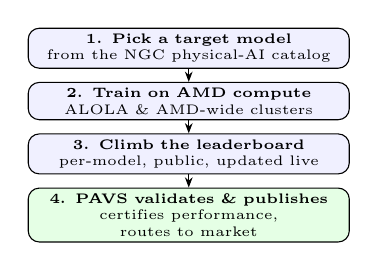
\begin{tikzpicture}[
  font=\tiny,
  box/.style={draw, rounded corners, align=center, text width=1.55in,
              minimum height=2.6ex, inner sep=2pt, fill=blue!6},
  final/.style={box, fill=green!10},
  arr/.style={-{Stealth[length=1.3mm]}}
]
\node[box] (pick) {\textbf{1. Pick a target model}\\ from the NGC physical-AI catalog};
\node[box, below=1.1ex of pick] (train) {\textbf{2. Train on AMD compute}\\ ALOLA \& AMD-wide clusters};
\node[box, below=1.1ex of train] (climb) {\textbf{3. Climb the leaderboard}\\ per-model, public, updated live};
\node[final, below=1.1ex of climb] (pub) {\textbf{4. PAVS validates \& publishes}\\ certifies performance, routes to market};
\draw[arr] (pick) -- (train);
\draw[arr] (train) -- (climb);
\draw[arr] (climb) -- (pub);
\end{tikzpicture}
\caption{The challenge mechanism: a known target, AMD compute, a public leaderboard, and PAVS certification --- repeated once per NGC model.}
\label{fig:mechanism}
\end{figure}

Why a challenge rather than a hire, or a single funded program? A challenge taps latent enthusiast engineering across all of AMD, rather than competing for headcount inside one already-stretched team. It converts a multi-year gap into many parallel short sprints, so progress does not wait on a single roadmap. And critically, no single business unit carries the bill --- the organization contributes cycles voluntarily, which is exactly the structural relief the deadlock in Section~\ref{sec:deadlock} requires.

%---------------------------------------------------------------------------
\section{The Target Set: 48 NGC Physical-AI Models Across Four Tiers}
\label{sec:targets}
%---------------------------------------------------------------------------

Of 125 NGC catalog entries scanned, 48 physical-AI models cannot carry over to AMD as-is and constitute the challenge's target list, organized into four priority tiers by deployment frequency and strategic relevance (Table~\ref{tab:tiers}; full per-model function and rationale in Appendix~\ref{app:tables}, Tables~\ref{tab:a1}--\ref{tab:a4}). Tier 1 and Tier 2 together --- 30 models --- are the actual "customer has this running on NVIDIA today and cannot move it" set, and represent the real switching-cost payoff described in Section~\ref{sec:switching}. Tier 3 and Tier 4 (18 models) matter chiefly if AMD also pursues the biometric/kiosk or HPC-climate verticals.

\begin{table}[H]
\centering
\caption{NGC physical-AI target set by priority tier.}
\label{tab:tiers}
\tiny
\begin{tabular}{@{}p{0.75in}p{0.2in}p{1.55in}@{}}
\toprule
Tier & \# & Focus \\
\midrule
1 --- Production perception & 10 & Metropolis/DeepStream: detection, recognition/re-ID, segmentation, retail, behavior/pose, OCR \\
2 --- Robotics building blocks & 7 & Isaac ROS: stereo/3D, pose, segmentation, pretrained backbones \\
3 --- Biometric/human-sensing & 12 & Face, gaze, emotion, gesture, heart-rate, inspection \\
4 --- Enterprise vision \& HPC/climate & 8 & Industrial inspection, PhysicsNeMo climate checkpoints \\
\bottomrule
\multicolumn{3}{l}{\textbf{Total: 48} of 125 NGC models scanned; 49 already portable; 28 unresolved.} \\
\end{tabular}
\end{table}

The pieces to close this gap already exist inside AMD; what is missing is organized, incentivized effort pointed at AMD silicon, not new invention.

%---------------------------------------------------------------------------
\section{Incentive Design: Every Party Wins by Playing}
\label{sec:incentive}
%---------------------------------------------------------------------------

A challenge sustains itself only if every party gains something by participating. This mechanism is designed so that three parties do (Table~\ref{tab:incentive}).

\begin{table}[H]
\centering
\caption{Incentive alignment across the three parties.}
\label{tab:incentive}
\tiny
\begin{tabular}{@{}p{0.62in}p{1.9in}@{}}
\toprule
Party & What they gain \\
\midrule
Participant (engineer) & Recognition and a top-team webpage listing; a countable contribution to their AMD record; an extra purpose alongside the day job; enthusiast hours converted into productive, citable output. \\
Organizer (PAVS) & Becomes the customer gateway for physical AI across AMD; reproducing models builds working ties across many teams; establishes PAVS as the lead player in a well-defined niche; bridges AMD's otherwise siloed physical-AI islands. \\
AMD (the organization) & The ecosystem gap closes on a compressed timeline against a known target; a growing pool of curated datasets and models compounds --- one team's output catalyzes the next; idle compute (ALOLA and others) is popularized; a pipeline of market-ready, AMD-native models results; all without a single-business-unit budget line. \\
\bottomrule
\end{tabular}
\end{table}

%---------------------------------------------------------------------------
\section{PAVS as the Customer Gateway to Physical AI}
\label{sec:pavs}
%---------------------------------------------------------------------------

Organizing the challenge is not overhead for PAVS --- it is how PAVS earns its position as the customer-facing entry point for physical AI at AMD. PAVS's commitment under this proposal is fourfold: issue an org-wide call for the right technical solutions; take the solutions that reach the bar to market; reproduce, evaluate, and certify each model and its performance; and curate the leaderboard and the per-model webpage that makes progress visible to the rest of the organization and to customers.

That commitment compounds into a structural role. By being the point through which every physical-AI solution enters, PAVS becomes the gateway; by reproducing and routing models across previously disconnected teams, it becomes the bridge connecting AMD's physical-AI islands; and by being first and most consistently present in this niche, it becomes the lead player within it. The organizing work is the mechanism by which PAVS earns the relationships and the position needed to route physical AI to market on AMD silicon.

%---------------------------------------------------------------------------
\section{Market Opportunity}
\label{sec:market}
%---------------------------------------------------------------------------

The prize is large enough to justify the organizing effort (Table~\ref{tab:market}). AMD's own projection puts the physical-AI silicon market at \$200B by 2035. Robotics startup funding reached \$22.2B in 2025, up 69\% year-over-year --- evidence that the buyers of tomorrow are being formed now, while their stacks are still being written. And the zero ROCm mentions across 1{,}228 ICLR 2026 VLA papers (Section~\ref{sec:moat}) is not only a symptom of the gap; it is a measure of how wide open the on-ramp still is to claim.

\begin{table}[H]
\centering
\caption{Sizing the opportunity.}
\label{tab:market}
\tiny
\begin{tabular}{@{}lc@{}}
\toprule
Metric & Figure \\
\midrule
Projected physical-AI silicon market (2035) & \$200B \\
Robotics startup funding (2025) & \$22.2B (+69\% YoY) \\
VLA papers at ICLR 2026 mentioning ROCm & 0 of 1{,}228 \\
\bottomrule
\end{tabular}
\end{table}

Make the transfer seamless --- a drop-in AMD replica for every model a customer already runs --- and AMD's price-performance is finally evaluated on its merits. The cheaper stack wins the deals it loses today, not because the silicon changed, but because the customer can finally afford to look at it.

%---------------------------------------------------------------------------
\section{Competitive Analysis}
\label{sec:competitive}
%---------------------------------------------------------------------------

\subsection{AMD vs.\ NVIDIA}
NVIDIA's moat, as established in Section~\ref{sec:moat}, is the vertically integrated model-to-simulation pipeline (NGC $\rightarrow$ TensorRT $\rightarrow$ Isaac ROS $\rightarrow$ cuRobo $\rightarrow$ Isaac Sim $\rightarrow$ Cosmos) and the developer base trained on it. AMD's structural counter is inference and total-cost-of-ownership economics that are already competitive (Section~\ref{sec:paradox}) combined with a target list that is public rather than proprietary --- NVIDIA's own catalog tells AMD exactly what to build. AMD does not need to out-invent NVIDIA's model zoo; it needs to reproduce the subset customers actually depend on (Tier 1 and Tier 2, Section~\ref{sec:targets}) faster than the switching-cost calculus in Section~\ref{sec:switching} continues to favor the incumbent.

\subsection{The Gap AMD Can Exploit}
The exploitable gap is not technical parity in isolation --- it is the absence of a routed, certified, drop-in replacement path. Three conditions make this window closeable rather than permanent: the target models and their performance bars are public (Section~\ref{sec:insight}); the compute to train replicas already exists inside AMD (ALOLA and AMD-wide clusters); and the research community defining the next generation of physical-AI models (VLA papers, Section~\ref{sec:moat}) has not yet locked in against AMD --- it simply is not aware AMD is an option. Every quarter this window stays open, NVIDIA's ecosystem depth increases and the switching-cost barrier in Section~\ref{sec:switching} compounds.

%---------------------------------------------------------------------------
\section{Strategic Recommendations and Roadmap}
\label{sec:reco}
%---------------------------------------------------------------------------

Table~\ref{tab:roadmap} sequences the challenge's rollout by effort and horizon: establish the mechanism and the first leaderboards quickly (near-term, largely organizational), prove out Tier 1 and Tier 2 replicas where the switching-cost payoff is largest (medium-term), and extend to Tier 3/4 only if the biometric or HPC-climate verticals become strategic priorities (long-term).

\begin{table}[H]
\centering
\caption{Staged rollout of the AMD-wide model challenge.}
\label{tab:roadmap}
\tiny
\begin{tabular}{@{}p{1.3in}p{0.55in}p{0.6in}@{}}
\toprule
Action & Horizon & Owner \\
\midrule
Org-wide announcement \& leaderboard platform & 0--1 mo & PAVS \\
Per-model GitHub repos, first 10 Tier-1 targets & 1--2 mo & PAVS + volunteers \\
Compute allocation (ALOLA \& AMD-wide) & 0--1 mo & Infrastructure \\
First leaderboard cycle \& winner publication & 2--4 mo & PAVS \\
Full Tier 1 + Tier 2 coverage (30 models) & 6--12 mo & Org-wide participants \\
Customer-facing certification \& routing & Ongoing from mo.\ 3 & PAVS \\
Tier 3/4 extension (conditional on vertical priority) & 12--24 mo & PAVS + BU sponsors \\
\bottomrule
\end{tabular}
\end{table}

%---------------------------------------------------------------------------
\section{The Ask}
\label{sec:ask}
%---------------------------------------------------------------------------

The plan is already staffed; what is missing is the mandate to start. From leadership, the request is a single, low-cost, high-leverage action: an org-wide email endorsing the challenge, the signal that gives the effort the traction a purely bottom-up initiative cannot generate on its own. Everything the challenge needs to run is already committed --- compute access has been granted (ALOLA and AMD-wide clusters), the per-model GitHub infrastructure is being created, and a team is already in place to drive the work day to day. Known target, staffed team, available compute: all that remains is the go-ahead.

%---------------------------------------------------------------------------
\section{Conclusion}
\label{sec:conclusion}
%---------------------------------------------------------------------------

AMD wins the spec sheet and still loses the deal, because the customer's decision was made one layer above the silicon --- inside an NVIDIA-built model and pipeline ecosystem that costs 6--18 engineer-months per deployment to leave. No single AMD business unit can close that gap inside a normal ROI window, because the payoff is multi-year and the work is, on its face, open-ended. The reframing in this paper removes that obstacle: because NGC's physical-AI models are named and their performance targets are public, closing the gap is bounded replication work, not open research, and history --- ImageNet, the DARPA Grand Challenge, the Netflix Prize --- shows that a scored, public target reliably converts exactly this kind of diffuse capability gap into fast, cheaply sourced progress. The proposal is concrete and already resourced: an AMD-wide, PAVS-organized model training challenge against the 48-model, four-tier NGC target set, with compute already granted and a team already in place. The market reward for closing this gap --- a projected \$200B physical-AI silicon market by 2035, and a wide-open on-ramp evidenced by zero ROCm mentions in 1{,}228 ICLR 2026 VLA papers --- is large and still unclaimed. What stands between AMD and that opportunity is not silicon, and not invention. It is the organizational go-ahead to point engineering cycles the organization already has at a target the organization already knows.

\textbf{Limitations.} The market-size, developer-population, and paper-count figures cited throughout rest on AMD's internal physical-AI market analysis and public catalog scans rather than a third-party audited dataset; the engineer-month and artifact-count switching-cost estimates in Section~\ref{sec:switching} are directional, drawn from deployment experience rather than a controlled study. The challenge mechanism, leaderboard platform, and PAVS certification process are proposed but not yet operated at scale, and their throughput and quality assumptions remain to be validated once the first leaderboard cycle completes.

\appendix
\section{Full NGC Physical-AI Target Set}
\label{app:tables}

\begin{table}[H]
\centering
\caption{Tier 1 --- Production Perception Stack (NVIDIA Metropolis/DeepStream). Highest priority: the most commonly deployed NGC models a customer runs today and cannot carry over to AMD.}
\label{tab:a1}
\tiny
\begin{tabular}{@{}p{0.85in}p{0.75in}p{0.75in}@{}}
\toprule
NVIDIA model & Function & Why it matters \\
\midrule
TrafficCamNet & Vehicle detection (traffic cameras) & Core Metropolis/smart-city SKU \\
PeopleNet / PeopleNet-AMR & Person detection & Most widely deployed DeepStream model \\
LPRNet + LPDNet & Plate detection + recognition pair & Sold as a pair, tolling/parking/security \\
VehicleMakeNet / VehicleTypeNet & Vehicle attribute classification & Paired with TrafficCamNet in the same pipelines \\
ReIdentificationNet (+ Transformer) & Person re-identification across cameras & Retail/security analytics \\
PeopleSemSegNet / AMR & Person segmentation & Privacy-masking, robotics safety zones \\
Retail Object Detection / Recognition & Shelf/product detection & Retail analytics vertical \\
Action Recognition Net & Action/behavior classification & Security, workplace safety \\
BodyPoseNet / PoseClassificationNet & Human pose estimation & Robotics, ergonomics, fitness \\
OCDNet / OCRNet & Scene text OCR & Logistics, document/label reading \\
\bottomrule
\end{tabular}
\end{table}

\begin{table}[H]
\centering
\caption{Tier 2 --- Robotics/Perception Building Blocks (Physical AI). The models Isaac ROS perception pipelines are built on --- closest to AMD-ROS/AARTS. Tier 1 + Tier 2 = 30 models, the real ``customer has this running and can't move it'' set.}
\label{tab:a2}
\tiny
\begin{tabular}{@{}p{0.95in}p{1.4in}@{}}
\toprule
NVIDIA model & Function \\
\midrule
Bi3D Proximity Segmentation & Stereo-based obstacle proximity \\
ESS DNN Stereo Disparity & Stereo depth \\
FoundationPose & 6-DoF object pose estimation/tracking \\
PointPillarNet & LiDAR 3D object detection \\
Transfusion (3D Object Detection) & Camera+LiDAR fusion detection \\
CitySemSegFormer & Semantic segmentation (autonomy/city-scale) \\
TAO Pretrained (Classification/DetectNet V2/EfficientDet/Instance Seg/Semantic Seg) & Generic backbones customers fine-tune on top of --- AMD needs some pretrained backbone family here or customers cannot start a TAO-style workflow on AMD \\
\bottomrule
\end{tabular}
\end{table}

\begin{table}[H]
\centering
\caption{Tier 3 --- Biometric/Human-Sensing (smaller but sticky niche). Matters mainly if AMD is also chasing the biometric/kiosk vertical.}
\label{tab:a3}
\tiny
\begin{tabular}{@{}p{0.95in}p{1.4in}@{}}
\toprule
NVIDIA model & Function \\
\midrule
FaceNet & Face detection \\
FaceDetectIR & Face detection (infrared) \\
GazeNet & Gaze tracking \\
EmotionNet & Emotion classification \\
GestureNet & Hand/body gesture recognition \\
HeartRateNet & Remote heart-rate estimation \\
Facial Landmark Estimator (FPENet) & Facial landmark detection \\
Deformable DETR (NvImageNet weights) & Detection backbone \\
FAN (NVImageNet weights) & Classification backbone \\
GCViT (NVImageNet weights) & Classification backbone \\
Visual ChangeNet Classification & Change detection classification \\
NVIDIA Optical Inspection Model & Industrial visual inspection \\
\bottomrule
\end{tabular}
\end{table}

\begin{table}[H]
\centering
\caption{Tier 4 --- Enterprise Vision \& HPC/Climate (lowest priority). Matters mainly if AMD is also chasing the enterprise-vision or HPC-climate vertical.}
\label{tab:a4}
\tiny
\begin{tabular}{@{}p{0.85in}p{0.75in}p{0.75in}@{}}
\toprule
NVIDIA model & Function & Why lower priority \\
\midrule
PCB Defect Classification & Industrial inspection & NVIDIA AI Enterprise EULA; small footprint \\
PeopleSemSegFormer & Person segmentation & NVIDIA AI Enterprise EULA; small footprint \\
DINO (NvImageNet weights) & Classification backbone & NVIDIA AI Enterprise EULA; small footprint \\
PhysicsNeMo: AFNO\_DX\_FI-V1-ERA5 & Weather forecasting & Community Model License; HPC/climate-only \\
PhysicsNeMo: AFNO\_DX\_SR-V1-ERA5 & Weather forecasting & Community Model License; HPC/climate-only \\
PhysicsNeMo: AFNO\_DX\_TP-V1-ERA5 & Weather forecasting & Community Model License; HPC/climate-only \\
PhysicsNeMo: AFNO\_DX\_WG-V1-ERA5 & Weather forecasting & Community Model License; HPC/climate-only \\
PhysicsNeMo: DLESyM-V1-ERA5 & Weather forecasting & Community Model License; HPC/climate-only \\
\bottomrule
\end{tabular}
\end{table}

48 models across four tiers, out of 125 scanned on NGC --- the remaining 77 are either already portable (49) or unresolved catalog entries (28).

\begingroup
\let\itshape\upshape
\bibliographystyle{abbrv}
\bibliography{refs}
\endgroup

\end{document}
